\documentclass[journal]{IEEEtran}

\ifCLASSINFOpdf
\else
   \usepackage[dvips]{graphicx}
\fi
\usepackage{url}

\hyphenation{op-tical net-works semi-conduc-tor}

\usepackage{graphicx}


\begin{document}

\title{Naturalization of Text by the Insertion of Pauses and Filler Words}

\author{Richa Sharma, Parth Vipul Shah, Ashwini M. Joshi 
\thanks{Manuscript first submitted on - 15-09-2020; No financial support; All authors have contributed equally.}
\thanks{Richa Sharma, is with the Department of Computer Science and Engineering, PES University, Bangalore, Karnataka 560085 India.}
\thanks{Parth Vipul Shah is with the Department of Computer Science and Engineering, PES University, Bangalore, Karnataka 560085 India.}
\thanks{Ashwini M. Joshi is a professor with the Department of Computer Science and Engineering, PES University, Bangalore, Karnataka 560085 India.}
}

\markboth{IEEE Signal Processing Letters, August 2020}
{Shell \MakeLowercase{\textit{et al.}}: Bare Demo of IEEEtran.cls for IEEE Journals}
\maketitle

\begin{abstract}

\end{abstract}

\begin{IEEEkeywords}

\end{IEEEkeywords}

\IEEEpeerreviewmaketitle

\section{Introduction}

% Motivation - 1
\IEEEPARstart{E}{lectronic} systems that interact with humans are making their way into everyday life. From robots in the house to personal assistants on our phones, these systems aid us in completing both simple and complex tasks. Interfacing with these electronic systems has also evolved. The focus has shifted to voice-based interactions over the more traditional text-based interactions seen in legacy systems. Voice commands and feedback provide a more natural way for us to interface with these systems. However, even with the rapid development of state of the art systems, we still largely interact with computerized voices. With this increase in voice-based interaction, we propose a set of methods to naturalize them. Naturalization of speech can be achieved in multiple ways but this letter focuses on the transformation of text by the addition of pauses and filler words such as 'uh' and 'um'. Google's Duplex can make calls on your behalf to book appointments or reserve tables and was unveiled in 2018. Despite being a computerized voice, pauses and filler words make the conversation more natural. Motivated by this observation, we propose a module that can be a part of a pipeline of posing a voice query to receiving a voice response from a system. This module takes the response text as input and outputs naturalized text which can then be input to a text-to-speech (TTS) module. Hence, this module naturalizes speech. \\

% Motivation - 2
Previous cognitive studies of natural human speech indicate that the addition, deletion, modification of words, sentences of standard speech are observed in conversations. These can be termed as disfluencies in speech. To achieve naturalization of speech, we resort to the addition of pauses and filler words such as 'uh' and 'um'. These pauses and filler words are an important part of natural conversations and unconsciously end up as a part of them. In natural conversations, pauses and filler words are often used when a conversationalist is either emphasizing on a part of the conversation or gathering their thoughts. By inserting them in standard text, the text is transformed into a more natural text. An example

\noindent\fbox{%
    \parbox{\linewidth}{%
       Standard Text: Let's see, Susan is 15. Aundrea is 9. Every stupid cliche you hear about kids, they change your life, they make you a better person, they make you whole, it's all true! Now I get it. \\
       Transformed Text: (um) Let's see (pause) Susan is 15. Aundrea is 9. Every stupid cliche you hear about kids, (pause) they change your life, they make you a better person, they make you whole, (pause) it's all true! Now (pause) I get it.
    }%
}
\\

% Previous works and novelty in this letter
As observed, in a conversational context, the transformed text sounds more natural than the standard text. Previously, in \cite{stolcke1} a language model is developed that predicts disfluencies probabilistically and uses an edited, fluent context to predict the following words. In \cite{stolcke2} a combination of prosodic cues modeled by decision trees and word-based event N-gram language models automatically detects disfluencies. These models detect disfluencies such as pauses and filler words in speech. In \cite{sundaram} an empirical text transformation method is proposed for spontaneous speech synthesizers which is trained on transcribed lecture monologue. The novelty of this letter includes (a) using transcribed movie dialogues as training data, (b) a hybrid approach in inserting pauses and filler words to increase confidence, (c) tunable degree of naturalization, (d) blind survey to assert the quality of transformed text.

% Summary of Method
First, we discuss data preprocessing followed by the two proposed methods. The bigram method involves the storing of bigrams with a pause or a filler word and its corresponding frequency in the training data. During transformation, a probabilistic approach is adopted to insert an appropriate pause or filler word. The hybrid approach first transforms text using the bigram method. A sequence to sequence model tuned to the context is then employed to validate these insertions.

\section{Method}
\subsection{Data}
The closest imitation of natural speech which is well recorded is in the form of dialogues from movie scripts. We use the Cornell University, Movie Dialogue Corpus on Kaggle\cite{cornell} as well as the Baskin Engineering, UC Santa Cruz, Film Corpus 2.0.\cite{ucsc} Combined, this forms a corpus of over $2.2 \times 10^{6}$ lines of text. Out of this, the lines containing disfluencies such as pauses and "uh", "um" are extracted. Two or more periods or dashes are also considered as pauses. Identified pauses are replaced by "(pause)" and "uh", "um" are replaced by "(uh)", "(um)" to maintain uniformity. This forms a corpus of over $2 \times 10^{5}$ lines and serves as the training data.

\subsection{Bigrams}

A sentence is taken as an input and the transformed sentence with the inserted pauses and filler words is output. Parameters that control the degree of naturalization can be set. Following are the steps of this method.

\begin{enumerate}
    \item A list of bigrams of words combined with pauses and filler words as predecessor or successor is constructed from the training data. The frequency of these bigrams is recorded. Additionally, a special token is appended at the start of each sentence to account for the possibility of an insertion at the beginning of the sentence.
    \item Clean the input sentence by dropping punctuation and numbers. Case is uniformly set to lower. 
    \item Find all possible insertions in the input sentence by splitting it into bigrams and comparing the predecessor and successor with the list of bigrams from step 1. This is the draw set, $D$.
    \item Draw a subset from $D$ based on the degree of naturalization and a probability distribution. The degree of naturalization is said to be the percentage of inserted words given the length of the input sentence.
    \begin{equation}
        \textit{Degree of naturalization} = \frac{\textit{Number of inserted words}}{\textit{Length of input sentence}}
    \end{equation}
    A probability distribution that fits the frequency of bigrams from step 1 is used to construct a subset of $D$. The set of probabilities, $P$ with which a bigram appears in a subset of $D$ is 
    \begin{equation}
        % P(x) = \frac{f(x)}{size(D)}
        P = \{\frac{f(x)}{size(D)}, \forall x \in D\}
    \end{equation}
    where $f(x)$ is the frequency of the bigram in the training data and $size(D)$ is the size of set $D$. The size of the subset of $D$ depends on the degree of naturalization.
    An uniform or any other probability distribution can be used too. The preceding distribution was used in this method as it gave the most intelligible transformations.  
    \item Construct the output sentence by adding the bigrams (filler word included) that are part of the subset of $D$ from step 4 to the input sentence.
\end{enumerate}

It is observed that some bigrams occur more frequently than others in a corpus of text. This is a property of natural speech that we leverage to output more intelligible transformations using the probability distribution mentioned in Equation 2. Step 1 can be performed independently and pre-computed before the method sees an input sentence. Therefore, this step does not contribute to the overall speed of the transformation. Table \ref{tab1} lists the five most frequently occurring bigrams from the training data.

\begin{table}
\caption{Most frequently occurring bigrams and their frequencies in the training data.}
\label{tab1}
\small
\setlength{\tabcolsep}{3pt}
\begin{tabular}{|p{80pt}|p{80pt}|p{80pt}|}
\hline
Predecessor& 
Successor& 
Frequency \\
\hline
(pause) & I & 13062\\
(pause) & and & 8364\\
you & (pause) & 4533\\
and & (uh) & 100\\
(uh) & I & 88\\
\hline
\end{tabular}
\label{tab1}
\end{table}

A valid subset of $D$ may not be possible if the training data has no occurrence of the bigrams present in the input sentence. Therefore, we propose a fallback method based on Parts of Speech (POS) tagging. This method is a variation of the method proposed above. A layer of abstraction is added by which the POS tag\cite{pos} of the training data and input sentence are considered for constructing the bigrams. However, this leads to a significant delay in transformation as the input sentence is first tagged.

\subsection{Hybrid}

Instead of probabilistically choosing a subset of $D$, in this method, the insertions are confirmed using a Recurrent Neural Network (RNN). The RNN predicts the next word based on substrings of the input sentence, a seed phrase. If the predicted word matches a filler word, it is inserted in the output sentence. The RNN is trained on the the training data. To train the model

\begin{enumerate}
    \item Pre-process the training data. 500 of the most representative sentences of corpus are selected as training data.
    \item Instantiate a tokenizer. The tokenizer converts the input data text into sequences. The sequence length is set to 3. The method uses the context of the two preceding words to predict one word.  
    \item The sequences are converted to categorical data and an RNN is trained using parameters defined in Table \ref{tab4}.
\end{enumerate}

\begin{table}
\caption{Architecture and Training Parameters of the Recurrent Neural Network (RNN).}
\label{tab4}
\small
\setlength{\tabcolsep}{3pt}
\begin{tabular}{|p{116pt}|p{116pt}|}
\hline
Parameter& 
Value \\
\hline
Layers &  1 \\
Units B & 100 LSTM\cite{lstm} \\
Loss Function &  Categorical Cross-entropy\cite{cce} \\
Optimizer &  Adam\cite{adam} \\
Epochs & 300 \\
\hline
\end{tabular}
\label{tab4}
\end{table}

We use a simple model as this ensures transformation speed is high. The training data consists of only a subset of the corpus because for larger training data, a drop in accuracy is observed as the simple model fails to fit the large sample space. A sequence length of 3 was found to give highest accuracy. This simple model can be improved to obtain more intellegible transformations.
To transform an input sentence after training is complete

\begin{enumerate}
    \item Clean the input sentence by dropping punctuation and numbers. Case is uniformly set to lower.
    \item From the bigram method, obtain the draw set, $D$. However, discard all bigrams that have a filler word as a predecessor.
    \item A substring of the input sentence constructed upto an insertion from $D$ is passed through the model to predict the next word. If the next word is the filler word from the bigram, the insertion is confirmed. This is the intermediate output. Based on the degree of naturalization, a subset of all confirmed insertions are selected and the output sentence is constructed.
\end{enumerate}

Sample incorrect and correct predictions for an input sentence "Let us try this one more time." follow
\noindent\fbox{%
    \parbox{\linewidth}{%
        Substring of the input sentence: Let \\
        Bigram from $D$: let, \textit{(pause)} \\
        Hybrid predicted next word: \textit{me}\\
        \textbf{Incorrect Prediction} \\
        Intermediate output: Let us try this one more time.
    }%
}
\\
\noindent\fbox{%
    \parbox{\linewidth}{%
        Substring of the input sentence: Let us\\
        Bigram from $D$: us, \textit{(pause)} \\
        Hybrid predicted next word: \textit{(pause)}\\
        \textbf{Correct Prediction} \\
        Intermediate output: Let us (pause) try this one more time.
    }%
}
\\

We observe that the model confirms a pause more frequently than the other filler words. According to \cite{cognitive}, pauses in natural language can be replaced by other filler words. Longer sentences are also more likely to begin with these filler words. Therefore, we take the liberty to replace the first $n$ pauses by the other filler words where $n$ is based on the degree of naturalization. 

After detailing the proposed methods, we state that richer training data is a sure way to output more intelligible transformations because the proposed methods rely heavily on the training data to generate possible insertions. Richer training data can be obtained by including a range of contexts if the input sentences are going to be general purpose. Training data can include specific contexts and introduce bias if the input sentences are going to be from a single context. Additionally, if the training data is a close representation of natural speech with the correct disfluencies inserted at the correct positions, the methods improve. 

\section{Results}

As there are multiple ways of achieving natural speech, we aim to transform the text into the most natural sounding version. To illustrate these multiple ways, following is an example

\noindent\fbox{%
    \parbox{\linewidth}{%
       Variation 1: This is (pause) the first time I am (uh) coming here. \\
       Variation 2: This is the (uh) first time (pause) I am coming here.\\
       Variation 3: This (uh) is the first time I am coming (pause) here.
    }%
}
\\

Therefore, we use a medium sized pool of 275 odd individuals to evaluate the outputs and determine if they sound natural or not. We refer to them as respondents hereafter. While answering the question "Which of the following sounds more natural?" judging between two text excerpts is more difficult than judging between two voice clips of the same text excerpts. Hence, the respondents were presented with two voice clips. One was a performance of an original interview's transcript, one was a performance of the transformed text of the same interview's transcript. Both were performed by the same voice actor. Here is an example of the output text from the bigram method followed by an example from the hybrid method


\noindent\fbox{%
    \parbox{\linewidth}{%
       Real: When we actually started recording the album we had this beautiful place, when we like rented this kind of beach (pause) shack and (um) that's the only thing I asked for in the budget though.\\
       Generated: When we actually started recording the (pause) album we had this beautiful place when we like rented this kind of beach shack (uh) and that's the (pause) only thing I asked for in the (pause) budget though.

    }%
}
\\


\noindent\fbox{%
    \parbox{\linewidth}{%
       Real: I spend a week in a year where I just go off and (uh) read (pause) people's PhD theses and new things that are going on in the field.\\
       Generated: I spend a week in a year where I just (uh) go off and read people's PhD theses and new things (uh) that are (pause) going on in the field.
    }%
}
\\

A "Cannot Determine" choice was also included as this would indicate near natural transformation by our methods. This was repeated twice per method with different interviews to test it's robustness when the context of the input text was varied. Table \ref{tab2} and \ref{tab3} list results of each sample, each method. Figures \ref{fig1} and \ref{fig2} illustrate only the summary for each method.

% TODO: add values to table, update figures

\begin{table}
\caption{Percentage of respondents determining the more natural sounding voice clip. Transformation method is bigram.}
\label{tab2}
\small
\setlength{\tabcolsep}{3pt}
\begin{tabular}{|p{58pt}|p{58pt}|p{58pt}|p{58pt}|}
\hline
Sample& 
Real& 
Generated&
Cannot Determine \\
\hline
% Sample A & 84 & 138 & 54 \\ % total: 276
% Sample B & 140 & 113 & 23 \\ % total: 276
Sample A & 30.4\% & 50.0\% & 19.6\% \\
Sample B & 50.7\% & 40.9\% & 8.3\% \\ 
\hline
\end{tabular}
\label{tab2}
\end{table}

\begin{table}
\caption{Percentage of respondents determining the more natural sounding voice clip. Transformation method is hybrid.}
\label{tab3}
\small
\setlength{\tabcolsep}{3pt}
\begin{tabular}{|p{58pt}|p{58pt}|p{58pt}|p{58pt}|}
\hline
Sample& 
Real& 
Generated&
Cannot Determine \\
\hline
% Sample C & 144 & 99 & 33 \\ % total: 276
% Sample D & 126 & 100 & 50 \\ % total: 276
Sample C & 52.2\% & 35.9\% & 12.0\% \\
Sample D & 45.7\% & 36.2\% & 18.1\% \\ 
\hline
\end{tabular}
\label{tab3}
\end{table}

\begin{figure}
\centerline{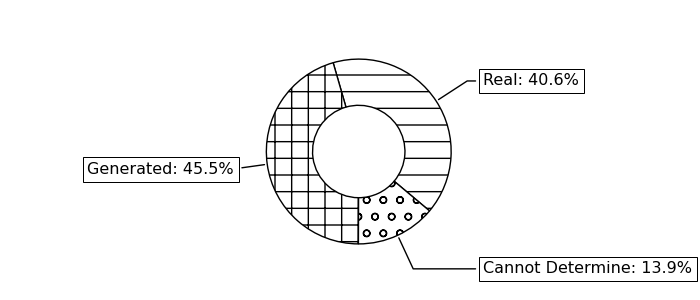
\includegraphics[width=\columnwidth]{bigram.png}}
\caption{Percentage of respondents determining the more natural sounding voice clip. Transformation method is bigram.}
\label{fig1}
\end{figure}

\begin{figure}
\centerline{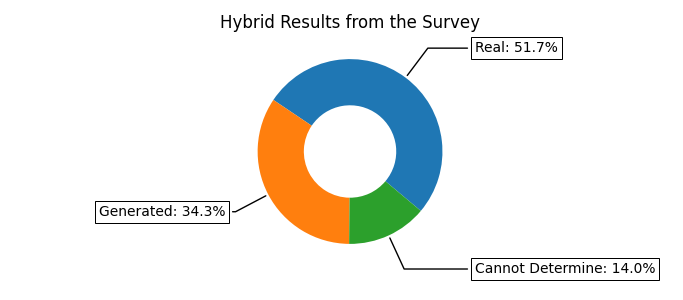
\includegraphics[width=\columnwidth]{hybrid.png}}
\caption{Percentage of respondents determining the more natural sounding voice clip. Transformation method is hybrid.}
\label{fig2}
\end{figure}

If "Generated" and "Cannot Determine" together form the majority of responses ($\geq 50\%$), our methods can be said to effectively naturalize text. The "Cannot Determine" choice indicates that the transformation was indiscernible from the original text. Counter-intuitively, the hybrid method performs slightly worse than the bigram method. However, this could be a result of the bias with respect to the context of the sample interviews. The methods may perform poorly in certain contexts. We reiterate that the methods are highly sensitive to the context of the training data. As the size of the training data and the breadth of the context increase, the methods get more robust and consequently, the transformations more natural. \\

As stated previously, our methods of text transformation are fast. This is to ensure that this text transformation module can be integrated as a precursor to a TTS module. Table \ref{tab5} details the timing data for both methods. All benchmarks are performed with equal compute power to maintain uniformity. 

% TODO: add justification for timing data and timing data

\begin{table}
\caption{Timing Data for the bigram and hybrid method.}
\label{tab5}
\small
\setlength{\tabcolsep}{3pt}
\begin{tabular}{|p{58pt}|p{58pt}|p{58pt}|p{58pt}|}
\hline
Sample& 
Real& 
Generated&
Cannot Determine \\
\hline
Sample C & \% & \% & \% \\
Sample D & \% & \% & \% \\
\hline
\end{tabular}
\label{tab5}
\end{table}

\section{Conclusion}

In this letter, we propose a novel, fast transformation method that has tunable naturalization. It also uses a hybrid approach to further confirm the transformations. We evaluate our methods using a medium sized pool of individuals to evaluate the outputs and determine if they are natural or not. We conclude that our methods yield near natural transformations of text and can be integrated as a module into a voice query to voice response pipeline.

% Hybrid approach for confirmation 
% Fast lookup for insertion of filler words
% Tunable naturalization
% Survey conducted to evaluate the accuracy of generated speech


\section*{References}

% \subsection*{Basic format for books:}

% J. K. Author, ``Title of chapter in the book,'' in {\em Title of His Published Book}, xth ed. City of Publisher, (only U.S. State), Country: Abbrev. of Publisher, year, ch. x, sec. x, pp. xxx--xxx.

% \subsection*{Examples:}
% \def\refname{}
% \begin{thebibliography}{34}

% \bibitem{}G. O. Young, ``Synthetic structure of industrial plastics,'' in {\em Plastics}, 2nd ed., vol. 3, J. Peters, Ed. New York, NY, USA: McGraw-Hill, 1964, pp. 15--64.

% \bibitem{}W.-K. Chen, {\it Linear Networks and Systems}. Belmont, CA, USA: Wadsworth, 1993, pp. 123--135.

% \end{thebibliography}

% \subsection*{Basic format for periodicals:}

% J. K. Author, ``Name of paper,'' Abbrev. Title of Periodical, vol. x,   no. x, pp. xxx--xxx, Abbrev. Month, year, DOI. 10.1109.XXX.123--456.

% \subsection*{Examples:}

% \begin{thebibliography}{34}
% \setcounter{enumiv}{2}

% \bibitem{}J. U. Duncombe, ``Infrared navigation Part I: An assessment of feasibility,'' {\em IEEE Trans. Electron Devices}, vol. ED-11, no. 1, pp. 34--39, Jan. 1959,10.1109/TED.2016.2628402.

% \bibitem{}E. P. Wigner, ``Theory of traveling-wave optical laser,''
% {\em Phys. Rev.},  vol. 134, pp. A635--A646, Dec. 1965.

% \bibitem{}E. H. Miller, ``A note on reflector arrays,'' {\em IEEE Trans. Antennas Propagat.}, to be published.
% \end{thebibliography}


% \subsection*{Basic format for reports:}

% J. K. Author, ``Title of report,'' Abbrev. Name of Co., City of Co., Abbrev. State, Country, Rep. xxx, year.

% \subsection*{Examples:}
% \begin{thebibliography}{34}
% \setcounter{enumiv}{5}

% \bibitem{} E. E. Reber, R. L. Michell, and C. J. Carter, ``Oxygen absorption in the earth’s atmosphere,'' Aerospace Corp., Los Angeles, CA, USA, Tech. Rep. TR-0200 (4230-46)-3, Nov. 1988.

% \bibitem{} J. H. Davis and J. R. Cogdell, ``Calibration program for the 16-foot antenna,'' Elect. Eng. Res. Lab., Univ. Texas, Austin, TX, USA, Tech. Memo. NGL-006-69-3, Nov. 15, 1987.
% \end{thebibliography}

% \subsection*{Basic format for handbooks:}

% {\em Name of Manual/Handbook}, x ed., Abbrev. Name of Co., City of Co., Abbrev. State, Country, year, pp. xxx--xxx.

% \subsection*{Examples:}

% \begin{thebibliography}{34}
% \setcounter{enumiv}{7}

% \bibitem{} {\em Transmission Systems for Communications}, 3rd ed., Western Electric Co., Winston-Salem, NC, USA, 1985, pp. 44--60.

% \bibitem{} {\em Motorola Semiconductor Data Manual}, Motorola Semiconductor Products Inc., Phoenix, AZ, USA, 1989.
% \end{thebibliography}

% \subsection*{Basic format for books (when available online):}

% J. K. Author, ``Title of chapter in the book,'' in {\em Title of Published Book}, xth ed. City of Publisher, State, Country: Abbrev. of Publisher, year, ch. x, sec. x, pp. xxx xxx. [Online]. Available: http://www.web.com 

% \subsection*{Examples:}

% \begin{thebibliography}{34}
% \setcounter{enumiv}{9}

% \bibitem{}G. O. Young, ``Synthetic structure of industrial plastics,'' in Plastics, vol. 3, Polymers of Hexadromicon, J. Peters, Ed., 2nd ed. New York, NY, USA: McGraw-Hill, 1964, pp. 15--64. [Online]. Available: http://www.bookref.com. 

% \bibitem{} {\em The Founders Constitution}, Philip B. Kurland and Ralph Lerner, eds., Chicago, IL, USA: Univ. Chicago Press, 1987. [Online]. Available: http://press-pubs.uchicago.edu/founders/

% \bibitem{} The Terahertz Wave eBook. ZOmega Terahertz Corp., 2014. [Online]. Available: http://dl.z-thz.com/eBook/zomega\_ebook\_pdf\_1206\_sr.pdf. Accessed on: May 19, 2014. 

% \bibitem{} Philip B. Kurland and Ralph Lerner, eds., {\em The Founders Constitution}. Chicago, IL, USA: Univ. of Chicago Press, 1987, Accessed on: Feb. 28, 2010, [Online] Available: http://press-pubs.uchicago.edu/founders/ 
% \end{thebibliography}

% \subsection*{Basic format for journals (when available online):}

% J. K. Author, ``Name of paper,'' {\em Abbrev. Title of Periodical}, vol. x, no. x, pp. xxx--xxx, Abbrev. Month, year. Accessed on: Month, Day, year, doi: 10.1109.XXX.123456, [Online].

% \subsection*{Examples:}

% \begin{thebibliography}{34}
% \setcounter{enumiv}{13}

% \bibitem{}J. S. Turner, ``New directions in communications,'' {\em IEEE J. Sel. Areas Commun.}, vol. 13, no. 1, pp. 11--23, Jan. 1995. 

% \bibitem{} W. P. Risk, G. S. Kino, and H. J. Shaw, ``Fiber-optic frequency shifter using a surface acoustic wave incident at an oblique angle,'' {\em Opt. Lett.}, vol. 11, no. 2, pp. 115--117, Feb. 1986.

% \bibitem{} P. Kopyt {\em et al.}, ``Electric properties of graphene-based conductive layers from DC up to terahertz range,'' {\em IEEE THz Sci. Technol.}, to be published. doi: 10.1109/TTHZ.2016.2544142.
% \end{thebibliography}

% \subsection*{Basic format for papers presented at conferences (when available online):}

% J.K. Author. (year, month). Title. presented at abbrev. conference title. [Type of Medium]. Available: site/path/file

% \subsection*{Example:}

% \begin{thebibliography}{34}
% \setcounter{enumiv}{16}

% \bibitem{}PROCESS Corporation, Boston, MA, USA. Intranets: Internet technologies deployed behind the firewall for corporate productivity. Presented at INET96 Annual Meeting. [Online]. Available: http://home.process.com/Intranets/wp2.htp
% \end{thebibliography}

% \subsection*{Basic format for reports  and  handbooks (when available online):}
  
% J. K. Author. ``Title of report,'' Company. City, State, Country. Rep. no., (optional: vol./issue), Date. [Online] Available: site/path/file 

% \subsection*{Examples:}

% \begin{thebibliography}{34}
% \setcounter{enumiv}{17}

% \bibitem{}R. J. Hijmans and J. van Etten, ``Raster: Geographic analysis and modeling with raster data,'' R Package Version 2.0-12, Jan. 12, 2012. [Online]. Available: http://CRAN.R-project.org/package=raster 

% \bibitem{}Teralyzer. Lytera UG, Kirchhain, Germany [Online]. Available: http://www.lytera.de/Terahertz\_THz\_Spectroscopy.php?id=home, Accessed on: Jun. 5, 2014.
% \end{thebibliography}

% \subsection*{Basic format for computer programs and electronic documents (when available online):}

% Legislative body. Number of Congress, Session. (year, month day). {\em Number of bill or resolution, Title}. [Type of medium]. Available: site/path/file
% {\em NOTE:} ISO recommends that capitalization follow the accepted practice for the language or script in which the information is given.

% \subsection*{Example:}

% \begin{thebibliography}{34}
% \setcounter{enumiv}{19}

% \bibitem{}U. S. House. 102nd Congress, 1st Session. (1991, Jan. 11). {\em H. Con. Res. 1, Sense of the Congress on Approval of Military Action}. [Online]. Available: LEXIS Library: GENFED File: BILLS 
% \end{thebibliography}

% \subsection*{Basic format for patents (when available online):}

% Name of the invention, by inventor’s name. (year, month day). Patent Number [Type of medium]. Available:site/path/file

% \subsection*{Example:}

% \begin{thebibliography}{34}
% \setcounter{enumiv}{20}

% \bibitem{}Musical tooth brush with mirror, by L. M. R. Brooks. (1992, May 19). Patent D 326 189
% [Online]. Available: NEXIS Library: LEXPAT File:   DES 

% \end{thebibliography}

% \subsection*{Basic format for conference proceedings (published):}

% J. K. Author, ``Title of paper,'' in {\em Abbreviated Name of Conf.}, City of Conf., Abbrev. State (if given), Country, year, pp. xxx--xxx.

% \subsection*{Example:}

% \begin{thebibliography}{34}
% \setcounter{enumiv}{21}

% \bibitem{}D. B. Payne and J. R. Stern, ``Wavelength-switched passively coupled single-mode optical network,'' in {\em Proc. IOOC-ECOC}, Boston, MA, USA, 1985,
% pp. 585--590.

% \end{thebibliography}

% \subsection*{Example for papers presented at conferences (unpublished):}

% \begin{thebibliography}{34}
% \setcounter{enumiv}{22}

% \bibitem{}D. E behard and E. Voges, ``Digital single sideband detection for inter ferometric sensors,'' presented at the {\em 2nd Int. Conf. Optical Fiber Sensors}, Stuttgart, Germany, Jan. 2--5, 1984.
% \end{thebibliography}

% \subsection*{Basic formatfor patents:}

% J. K. Author, ``Title of patent,'' U. S. Patent x xxx xxx, Abbrev. Month, day, year.

% \subsection*{Example:}

% \begin{thebibliography}{34}
% \setcounter{enumiv}{23}

% \bibitem{}G. Brandli and M. Dick, ``Alternating current fed power supply,'' U. S. Patent 4 084 217, Nov. 4, 1978.
% \end{thebibliography}

% \subsection*{Basic format for theses (M.S.) and dissertations (Ph.D.):}

% a) J. K. Author, ``Title of thesis,'' M. S. thesis, Abbrev. Dept., Abbrev. Univ., City of Univ., Abbrev. State, year.

% b) J. K. Author, ``Title of dissertation,'' Ph.D. dissertation, Abbrev. Dept., Abbrev. Univ., City of Univ., Abbrev. State, year.

% \subsection*{Examples:}

% \begin{thebibliography}{34}
% \setcounter{enumiv}{24}

% \bibitem{}J. O. Williams, ``Narrow-band analyzer,'' Ph.D. dissertation, Dept. Elect. Eng., Harvard Univ., Cambridge, MA, USA, 1993.

% \bibitem{}N. Kawasaki, ``Parametric study of thermal and chemical nonequilibrium nozzle flow,'' M.S. thesis, Dept. Electron. Eng., Osaka Univ., Osaka, Japan, 1993.
% \end{thebibliography}

% \subsection*{Basic format for the most common types of unpublished references:}

% a) J. K. Author, private communication, Abbrev. Month, year.

% b) J. K. Author, ``Title of paper,'' unpublished.

% c) J. K. Author, ``Title of paper,'' to be published.

% \subsection*{Examples:}

% \begin{thebibliography}{34}
% \setcounter{enumiv}{26}

% \bibitem{}A. Harrison, private communication, May 1995.

% \bibitem{}B. Smith, ``An approach to graphs of linear forms,'' unpublished.

% \bibitem{}A. Brahms, ``Representation error for real numbers in binary computer arithmetic,'' IEEE Computer Group Repository, Paper R-67-85.
% \end{thebibliography}

% \subsection*{Basic formats for standards:}

% a) {\em Title of Standard}, Standard number, date.

% b) {\em Title of Standard}, Standard number, Corporate author, location, date.

% \subsection*{Examples:}

% \begin{thebibliography}{34}
% \setcounter{enumiv}{29}


% \bibitem{}IEEE Criteria for Class IE Electric Systems, IEEE Standard 308, 1969.

% \bibitem{} Letter Symbols for Quantities, ANSI Standard Y10.5-1968.
% \end{thebibliography}

% \subsection*{Article number in reference examples:}

% \begin{thebibliography}{34}
% \setcounter{enumiv}{31}

% \bibitem{}R. Fardel, M. Nagel, F. Nuesch, T. Lippert, and A. Wokaun, ``Fabrication of organic light emitting diode pixels by laser-assisted forward transfer,'' {\em Appl. Phys. Lett.}, vol. 91, no. 6, Aug. 2007, Art. no. 061103. 

% \bibitem{} J. Zhang and N. Tansu, ``Optical gain and laser characteristics of InGaN quantum wells on ternary InGaN substrates,'' {\em IEEE Photon.} J., vol. 5, no. 2, Apr. 2013, Art. no. 2600111
% \end{thebibliography}

% \subsection*{Example when using et al.:}

% \begin{thebibliography}{34}
% \setcounter{enumiv}{33}

% \bibitem{}S. Azodolmolky {\em et al.}, Experimental demonstration of an impairment aware network planning and operation tool for transparent/translucent optical networks,'' {\em J. Lightw. Technol.}, vol. 29, no. 4, pp. 439--448, Sep. 2011.
% \end{thebibliography}

\end{document}
